% Workshop submission, 8 pages of content.
% Neutral article class: swap in the venue style file (neurips_2026.sty,
% iclr2027_conference.sty, colm2026.sty, ...) and delete the geometry line.
%
% Figures are built by ai_post_analysis/src/paper_figures.py (vector PDF, no
% baked-in titles). Build from inside this directory:
%     pdflatex format_implicit_purpose.tex   (twice, for \ref cross-references)
\documentclass[10pt]{article}
\usepackage[margin=1in]{geometry}
% Latin Modern is a scalable Type1 face; without it microtype's font expansion
% fails on a stock MiKTeX install ("auto expansion is only possible with
% scalable fonts"). Venue style files usually set this themselves.
\usepackage[T1]{fontenc}
\usepackage{lmodern}
\usepackage{amsmath,amssymb}
\usepackage{booktabs}
\usepackage{graphicx}
\usepackage{microtype}
\usepackage[hidelinks]{hyperref}
\usepackage{caption}
\captionsetup{font=small,labelfont=bf,skip=6pt}
\usepackage{titlesec}
\titlespacing*{\section}{0pt}{1.05em}{0.45em}
\titlespacing*{\subsection}{0pt}{0.75em}{0.3em}
\graphicspath{{figures/}}

\newcommand{\ci}[2]{{\footnotesize[#1,\,#2]}}

\title{\bfseries Format Carries Implicit Purpose,\\ but Probe Scores Overstate It}
\author{Anonymous submission}
\date{}

\begin{document}
\maketitle

\begin{abstract}
When a prompt states no purpose, does its \emph{presentation} tell the model
what kind of situation it is in? We measure the projection of purpose-neutral
prompts onto a probe direction fitted to explicitly stated response purpose, on
a fully crossed panel of 320 payload blocks $\times$ 13 templates $\times$
\{evaluation, deployment, no-cue\} extracted from three Llama checkpoints. We
report every effect in a calibrated unit: the effect of literally writing
\emph{``an auditor will inspect this response.''} Three results follow. (i)
Uncued prompts are not neutral --- they sit $0.20$--$0.39$ of the way from the
deployment centroid toward the evaluation centroid at mid-to-late depth. (ii)
The shift is \emph{specific to uncued prompts}: the same format contrast
measured on cued rows is near zero, and the cued-minus-uncued differential
excludes zero at every layer of all three models, which rules out a shared
per-template offset on the axis. (iii) Most importantly, a stricter test
disagrees with the probe. Asking whether the \emph{activation displacement
itself} aligns with the matched evaluation-minus-deployment displacement, we
find that benchmark-shaped prompting survives ($27/27$, $70/72$ and $69/71$
reliable layers with intervals excluding zero), while a serialization effect
that is robust under four probe estimators --- including one that reverses the
comparison contrast --- \emph{reverses sign} in one checkpoint and vanishes in
another. We conclude that probe-score drift and counterfactual displacement
alignment are different claims about a representation, and that the
eval-aware\-ness probing literature should report them separately. All results
are exploratory analyses of a frozen, hash-pinned activation set; the estimand
is a projection onto a stated-purpose axis, not evaluation awareness, behavior,
or causation.
\end{abstract}

\section{Introduction}

Two recent positions frame the question of whether language models know when
they are being tested. Needham et al.~\cite{needham2025} report that frontier
models often can tell evaluation transcripts from deployment transcripts,
establishing the phenomenon behaviorally. Devbunova~\cite{devbunova2026} raises
the deflationary reply: perhaps such probes read the \emph{wrapper} --- the
multiple-choice scaffolding, the option letters, the terse imperative --- and
not the situation. That reply has force, because prompt format is known to be
both enormously influential on behavior and highly linearly separable in
activation space~\cite{sclar2024}.

Both positions treat format as a \emph{confound}: something to control away, or
something that dissolves the phenomenon under scrutiny. We take a third
position. If a prompt's presentation reliably co-occurs with a kind of
situation in training data, then format is not noise contaminating a purpose
representation --- it is one of the channels through which purpose is conveyed.
The question is not whether format contaminates the probe, but \emph{how much
purpose a wrapper is worth}, and whether that quantity behaves like information
about the situation or like an artifact of the measuring instrument.

Answering this requires a design in which purpose and format are crossed by
construction, and a unit in which the answer is interpretable. We supply both.
Our contrast set holds payload content fixed inside every comparison, balances
the cue stratum so the probe direction is trained decorrelated from format, and
scores held-out cue vocabulary the probe never saw. Every effect is then
divided by the effect of the explicit purpose sentence at the same layer, so
that a coefficient of $0.25$ reads as \emph{``this wrapper is worth a quarter of
telling the model an auditor is watching.''}

The measurement produces a clean positive result and then, under a stricter
test, partially retracts one half of it. We report both, because the retraction
is the more transferable finding.

\paragraph{Contributions.}
\begin{enumerate}\itemsep1pt
\item A \textbf{calibrated unit} for format effects on purpose representation:
      every coefficient is expressed as a fraction of the explicit stated-purpose
      intervention, making effects comparable across layers, models and papers
      (\S\ref{sec:design}).
\item A \textbf{no-cue-specificity design}: measuring the same format contrast
      on cued and uncued rows and taking the difference cancels any per-template
      offset on the axis, separating ``format shifts the probe'' from ``format
      supplies purpose information'' (\S\ref{sec:specific}).
\item A \textbf{counterfactual geometry test} showing that a probe-score effect
      robust across three checkpoints, every layer, and four estimators can fail
      to correspond to a displacement in the same direction --- with a sign
      reversal in one checkpoint (\S\ref{sec:geometry}). This is a methodological
      caution for the probing literature that does not depend on our domain.
\end{enumerate}

\section{Related work and positioning}

\textbf{Evaluation awareness.} Needham et al.~\cite{needham2025} benchmark
black-box discrimination of evaluation from deployment. Our estimand is
representational and upstream of behavior: we never sample a response.

\textbf{The format-sensitivity deflation.} Devbunova~\cite{devbunova2026} argues
eval-awareness signals may reduce to format sensitivity.
\S\ref{sec:specific} is the direct reply: a nuisance direction picked up from
the wrapper would offset cued and uncued rows equally, and it does not. We also
re-analyzed that work's released activations under a common-item randomization
null and could not distinguish its wrapper-transfer penalty from the null
($p = 0.074$, 256 draws); we report this only as context for why we rebuilt the
design rather than extending it.

\textbf{Format sensitivity.} Sclar et al.~\cite{sclar2024} document spreads of
up to 76 accuracy points across semantically equivalent templates, near-perfect
internal separability of formats, and --- importantly for us --- \emph{weak
cross-model correlation} of format effects. We adopt their methodological
prescription (treat format as a sampled distribution of templates with declared
structural dimensions, report spread rather than a single coefficient) and we
confirm their warning: our per-template ordering correlates only moderately
across model scales ($r \approx 0.13$--$0.58$), so \emph{which} wrapper reads as
what is not a portable claim. Only the existence and calibrated magnitude of the
effect is.

\textbf{Control tasks.} Our permutation null follows Hewitt and
Liang~\cite{hewitt2019}: a probe of identical capacity fitted to a shuffled
target, which we find does \emph{not} produce a zero shift and therefore must be
the comparison baseline rather than zero.

\section{Design, probe, and calibration}
\label{sec:design}

\paragraph{Panel.} We use a frozen, sha256-pinned render of $11{,}520$ prompts:
$320$ payload blocks $\times$ $13$ templates $\times$ $3$ purpose conditions
(evaluation, deployment, no-cue), fully crossed. A \emph{payload block} is a
task instance; a \emph{template} is a wrapper that renders it. Because every
block appears under every template and every purpose condition, all contrasts
below are computed \emph{within} a payload block, so content is held fixed by
construction rather than by covariate adjustment.

Templates carry declared structural dimensions rather than a single categorical
label. Two cuts matter here. The \textbf{benchmark/casual} cut is the sampling
stratum --- which real-world source distribution a template is modeled on
(MMLU-style and BIG-bench-style scaffolds~\cite{hendrycks2021,srivastava2023} on
one side, conversational traffic on the other). The \textbf{serialization} cut
is orthogonal in intent: three of the thirteen templates render the prompt as a
machine-readable record (a JSON object with \texttt{input} and \texttt{choices}
fields and no instruction at all; an XML-tagged
\texttt{<question>}/\texttt{<options>} wrapper; a Markdown \texttt{\#\#\# Input}
document), while the rest address the model in prose. The design deliberately
breaks the naive alignments: one benchmark-stratum template is XML-serialized,
and conversational templates appear on the evaluation side, so ``MCQ
$\Rightarrow$ evaluation'' and ``JSON $\Rightarrow$ evaluation'' fail by
construction.

Evaluation and deployment renders of the same block under the same template are
\textbf{byte-identical twins} differing only in a one-sentence purpose cue, so
the calibration denominator is a pure single-sentence intervention. Cue
sentences are partitioned into five \textbf{vocabulary-disjoint folds}.

\paragraph{Probe.} \texttt{StandardScaler} $+$
\texttt{LogisticRegression($C{=}0.1$)} on the last-prompt-token residual stream
(zero-based transformer-block output before the final norm), trained on the
cued stratum, leave-one-cue-vocabulary-fold-out. The cued stratum is balanced
$3{,}840/3{,}840$ across purpose \emph{and} crossed with format, so the axis is
trained decorrelated from the format cut. No-cue rows carry no fold and are
scored by the mean of the five held-fold models. Held-fold purpose AUC is
$0.91$--$0.99$ (8B) and $0.91$--$1.00$ (70Bs).

\paragraph{Calibration.} Logistic decision values have arbitrary scale, so
every effect is divided by the stated-cue effect at the same layer:
\begin{align}
\Delta_{\text{stated}} &= \overline{\text{eval}} - \overline{\text{deploy}}
   \quad\text{(block means, out-of-fold)}\\
\pi(g) &= \big(\overline{\text{no-cue} \in g} - \overline{\text{deploy}}\big)
   \,/\, \Delta_{\text{stated}}\\
\rho &= \overline{\big(\text{no-cue bench} - \text{no-cue casual}\big)}
   \,/\, \Delta_{\text{stated}}
\end{align}
$\pi = 1$ means ``as far toward evaluation as writing the auditor sentence.''
Because every block appears in every condition, $\rho$ is a within-block paired
quantity. Where the axis itself is weak the ratio's denominator is unreliable,
so we grey out depths with purpose AUC $< 0.95$ in every figure.

\paragraph{Uncertainty.} Cluster bootstrap over the $320$ payload block ids,
$B = 10{,}000$, seed $0$, percentile 95\% intervals; numerator and denominator
are recomputed from the same resample so ratios retain their correlation.
Resampling items rather than blocks would understate uncertainty roughly
four-fold. BLAS is pinned to one thread per worker, without which the thread
count changes lbfgs summation order and moves AUC in the fourth decimal.

\paragraph{Models.} Llama-3.1-8B-Instruct ($32$ layers), Llama-3.1-70B-Instruct
and Llama-3.3-70B-Instruct ($80$ layers each), all at pinned revisions. The two
70Bs are architecturally identical and were run on the same byte-identical
prompts, differing only in post-training. We index depth by
$q = \text{layer}/(L-1)$ for cross-model comparison.

\section{Uncued prompts are not neutral, and format moves them}
\label{sec:drift}

Projected onto the purpose axis, prompts that state no purpose do not sit at the
deployment centroid. At mid-to-late depth $\pi_{\text{no-cue}}$ reaches
$0.20$--$0.29$ in the 8B and $0.27$--$0.39$ in both 70Bs: an uncued prompt is
already a fifth to two fifths of the way toward ``an auditor is watching.''

Format moves it, and the two cuts point in \emph{opposite directions}
(Figure~\ref{fig:depth}). The benchmark/casual contrast the literature uses is
real and points toward evaluation: $\rho$ is positive with intervals excluding
zero across essentially the whole reliable depth range of all three models. The
serialization contrast is negative just as consistently --- markup-wrapped
prompts sit closer to the \emph{deployment} pole. Being handed a
machine-readable record reads as production traffic, not as a test.

\begin{figure}[t]\centering
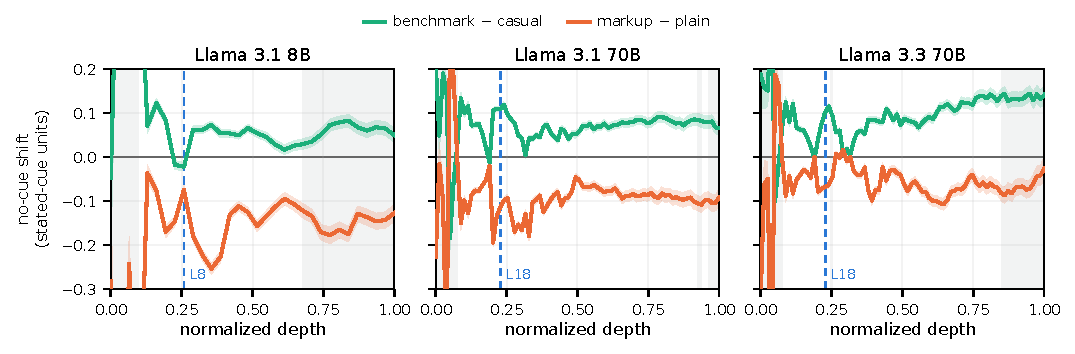
\includegraphics[width=\textwidth]{fig1_depth_profile.pdf}
\caption{Both format contrasts across depth, in calibrated stated-cue units,
with block-bootstrap 95\% bands. The benchmark contrast (green) is positive and
the serialization contrast (orange) negative at essentially every reliable layer
of all three checkpoints. Dashed line: peak-AUC layer. Grey: purpose
AUC $< 0.95$, where the ratio's denominator is unreliable.}
\label{fig:depth}
\end{figure}

The opposite sign replicates in all three checkpoints. The relative magnitude
does not: markup runs $2$--$4\times$ the benchmark contrast in the 8B but is
comparable to or smaller than it in the 70Bs. We therefore do not claim the
benchmark/casual cut is ``the wrong one'' --- only that it is not the only one,
and that a second cut of comparable size runs the other way.

\paragraph{Secondary observation: post-training.} The two 70Bs are a controlled
A/B on post-training alone. They are nearly indistinguishable through the first
half of the network, but from $\sim 50\%$ depth onward 3.3's
benchmark$\rightarrow$evaluation drift is $1.4$--$1.9\times$ larger with
non-overlapping intervals ($\rho = +0.079$ vs.\ $+0.134$ at $q = 0.76$), while
the markup contrast is similar in both --- visible in Figure~\ref{fig:depth} as
the green curve rising in the right panel but not the middle one. This is not a
normalization artifact: $\Delta_{\text{stated}}$ is uniformly $\sim 10\%$
\emph{smaller} in 3.3, including at early layers where $\rho$ matches. We flag
it as an observation only --- $n = 2$ checkpoints of one lineage.

\section{The shift exists only when no purpose is stated}
\label{sec:specific}

\S\ref{sec:drift} is vulnerable to a simple deflation: the purpose axis might
carry a per-template offset, so that markup templates score lower on it for
reasons having nothing to do with purpose. This is the deflationary reading
of~\cite{devbunova2026}, and it makes a testable prediction --- such an offset
would depress cued and uncued rows \emph{equally}.

It does not. Figure~\ref{fig:specific} measures the identical format contrast on
the cued rows and on the no-cue rows, both block-demeaned, in the same axis
units. The cued curve is pinned near zero at every depth in all three models;
the no-cue curve sits well below it; and their difference --- in which any
offset shared by cued and uncued rows cancels exactly --- is negative at
\emph{every layer of all three models} with intervals excluding zero
(Table~\ref{tab:diff}).

\begin{figure}[t]\centering
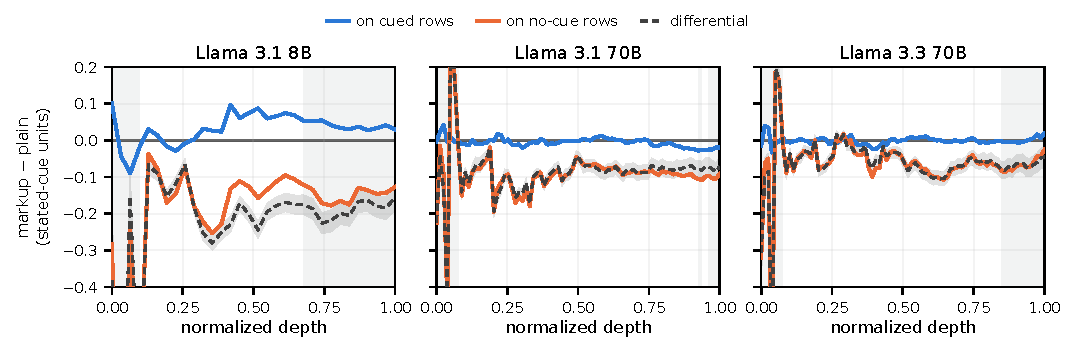
\includegraphics[width=\textwidth]{fig2_no_cue_specific.pdf}
\caption{The load-bearing control. The same markup $-$ plain contrast measured
on cued rows (blue) and no-cue rows (orange), with their differential (dashed,
95\% band). A per-template offset on the axis would move both curves together;
instead the cued curve stays at zero while the no-cue curve does not. Grey as in
Figure~\ref{fig:depth}.}
\label{fig:specific}
\end{figure}

\begin{table}[t]\centering\small
\caption{Anchor values for Figure~\ref{fig:specific}. A per-template axis offset
cancels in the differential column.}
\label{tab:diff}
\begin{tabular}{llccc}
\toprule
model & layer & cued & no-cue & differential \\
\midrule
3.1 8B  & 11 & $+0.026$ & $-0.254$ & $\mathbf{-0.280}$ \ci{-0.300}{-0.260}\\
3.1 8B  & 24 & $+0.041$ & $-0.178$ & $\mathbf{-0.219}$ \ci{-0.249}{-0.189}\\
3.1 70B & 30 & $-0.001$ & $-0.125$ & $\mathbf{-0.124}$ \ci{-0.136}{-0.111}\\
3.1 70B & 79 & $-0.020$ & $-0.091$ & $\mathbf{-0.071}$ \ci{-0.096}{-0.046}\\
3.3 70B & 40 & $+0.001$ & $-0.063$ & $\mathbf{-0.064}$ \ci{-0.081}{-0.046}\\
3.3 70B & 79 & $+0.019$ & $-0.026$ & $\mathbf{-0.045}$ \ci{-0.075}{-0.016}\\
\bottomrule
\end{tabular}
\end{table}

\textbf{This is the signature a prior should have}: the wrapper matters when the
prompt says nothing about purpose, and stops mattering once purpose is stated.
In the 8B the cued and no-cue per-template offsets are in fact \emph{negatively}
correlated across templates at most layers ($r \approx -0.3$ to $-0.67$), the
opposite of what a shared offset predicts.

\paragraph{Within-template replication.} Only $3$ of $13$ templates are
markup-serialized, so ``serialization'' is confounded with ``those three
templates.'' One factor escapes that confound: a response-contract slot rotates
over $4$--$5$ values \emph{inside} every template, one of which (\textsf{C4},
\emph{``return an object that has one field named answer''}) requests a
structured, machine-readable response. Under a two-way fixed-effects model
absorbing both payload block and template, \textsf{C4} reproduces the same
signature with no template confounding: 8B differential $-0.150$
\ci{-0.178}{-0.122} at L24 and $-0.195$ \ci{-0.221}{-0.167} at L28; 3.1-70B
$-0.116$ \ci{-0.139}{-0.093} at L70. \textbf{It does not hold in 3.3-70B}, where
the differential is negative early ($-0.051$ at L18), turns \emph{positive} at
L40 ($+0.042$ \ci{+0.024}{+0.058}), and is indistinguishable from zero from L50
on. We report this as a failure: the cleanest available escape from the template
confound replicates in two of three checkpoints. Note also that this test was
chosen \emph{after} seeing the markup result, making it a targeted prediction on
a non-confounded factor rather than independent confirmation.

\section{Probe drift is not displacement}
\label{sec:geometry}

Everything above is a statement about a \emph{scalar assigned by a fitted
probe}. A stronger and rarely-asked question is whether the activation
displacement itself points the same way as the matched purpose intervention.
For each payload block $b$ we form, on the $11$ non-legacy templates that make a
complete panel,
\[
P_b = \operatorname*{mean}_{t}\big(h^{\text{eval}}_{bt} - h^{\text{deploy}}_{bt}\big),
\qquad
V_{bt} = h^{\text{no-cue}}_{bt} - \tfrac12\big(h^{\text{eval}}_{bt} + h^{\text{deploy}}_{bt}\big),
\]
\[
D_b(g) = \operatorname*{mean}_{t \in g} V_{bt} - \operatorname*{mean}_{t \notin g} V_{bt},
\]
and report $\cos\!\big(\overline{P}, \overline{D}\big)$. The subtraction in $V$
removes the format displacement shared by cued and uncued rows before the cosine
is taken --- the vector-valued analogue of \S\ref{sec:specific}. Uncertainty is a
joint delete-one-block jackknife. A second estimator divides every feature by
its cued-row standard deviation, fits purpose directions excluding each cue
family in turn, and reports the held-family projection of $D$ as a fraction of
the explicit-purpose magnitude. We gate on representational stability: layers
where the excluded-fold and held-fold purpose directions have cosine $< 0.5$ are
excluded as unreliable ($5$ of $32$ in the 8B, $8$ and $9$ of $80$ in the 70Bs).

\begin{figure}[t]\centering
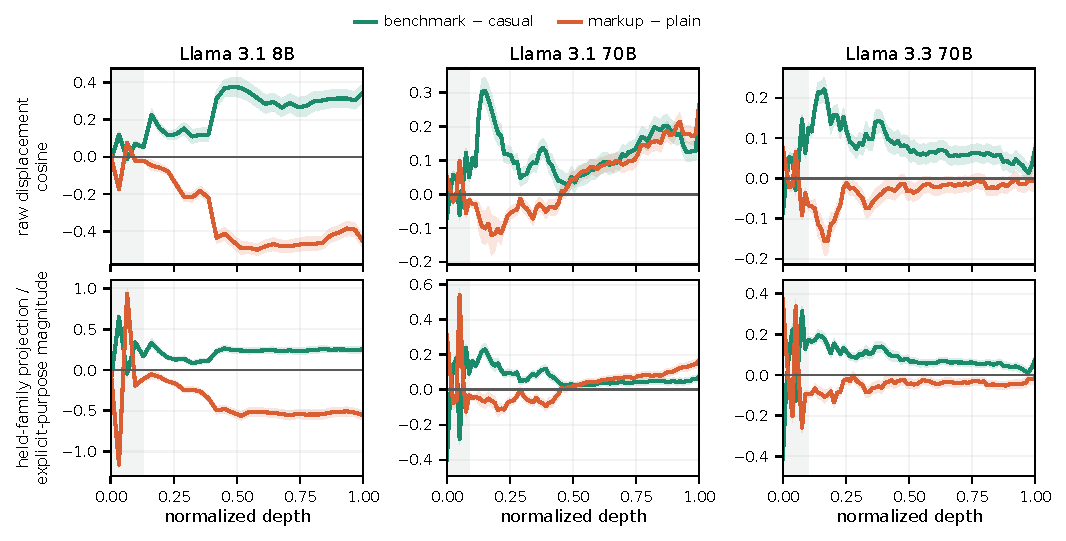
\includegraphics[width=\textwidth]{fig3_counterfactual_geometry.pdf}
\caption{The two contrasts diverge under the stricter metric. Top: raw
displacement cosine, joint block-jackknife 95\% intervals. Bottom: held-family
projection as a fraction of explicit-purpose magnitude. The benchmark contrast
(green) stays positive in all three checkpoints. The serialization contrast
(orange) is strongly negative in the 8B, \emph{crosses zero and ends positive}
in 3.1-70B, and decays to zero in 3.3-70B. Grey: cross-fitted purpose direction
unstable (held-vs-excluded cosine $< 0.5$), excluded from all counts.}
\label{fig:geom}
\end{figure}

\paragraph{Benchmark shaping survives the metric change.} Its raw alignment is
positive with a jackknife interval excluding zero at \emph{all} $27$ reliable 8B
layers, $70$ of $72$ in 3.1-70B, and $69$ of $71$ in 3.3-70B. At $q = 0.375$ the
raw cosines are $+0.120$ \ci{+0.083}{+0.156}, $+0.138$ \ci{+0.110}{+0.166} and
$+0.143$ \ci{+0.113}{+0.172} respectively. This upgrades the claim from ``the
probe scores these higher'' to ``the no-cue-specific benchmark displacement has
a component in the same full-space direction as explicitly stated evaluation.''

\paragraph{Serialization does not.} It is negative at every reliable 8B layer,
reaching $-0.488$ \ci{-0.523}{-0.454} at L16. But in 3.1-70B it is negative only
through L35, crosses zero at L36--L37, and is \emph{positive} from L38 through
L79, ending at $+0.262$ \ci{+0.229}{+0.296}. In 3.3-70B it stays weakly negative
and reaches zero at the end ($-0.004$ \ci{-0.034}{+0.026}). The middle panel of
Figure~\ref{fig:geom} is the crux: the orange curve climbs through the green one
at mid-depth, in a model where the probe-score differential
(Figure~\ref{fig:specific}) is negative at every layer. The score-based markup
differential therefore cannot be described as the whole activation displacement
moving toward deployment. In the 70Bs it is a \emph{component selected by the
probe metric}, while the dominant Euclidean displacement is checkpoint- and
depth-dependent.

\paragraph{An exact null over the template catalog.} Because the template set is
fixed and small, we enumerate every same-size partition of the $11$ templates
($\binom{11}{6} = 462$ for the benchmark cut, $\binom{11}{3} = 165$ for markup)
and ask where the \emph{named} grouping falls. The benchmark grouping is
unusually positive at $q = 0.25$ and $0.375$ in both 70Bs (two-sided
$p = 0.041$--$0.050$) but not at later depths and not in the 8B. The 8B markup
grouping is unusually negative under the directional test at mid and deep fixed
depths (one-sided $p = 0.006$--$0.012$), with the two-sided test crossing $0.05$
only at $q = 0.5$. Neither named grouping is a random sample from a format
population, and neither carries a strong population claim.

\paragraph{What this means.} A probe-score effect can be robust across three
checkpoints, every layer, and four estimators (\S\ref{sec:controls}) and still
fail to correspond to a displacement in the same direction. That is not a
statement about serialization; it is a statement about what a probe score
licenses. The probe finds a low-variance direction separating the classes it was
trained on and reports a projection onto it; the projection can move robustly
while the bulk of the displacement moves elsewhere or opposite. We recommend
that work in this area report probe drift and displacement alignment as separate
claims, and treat agreement between them as a result rather than an assumption.

\section{Controls and robustness}
\label{sec:controls}

\paragraph{Would any decodable axis do this?} \texttt{task\_family} is a property
of the payload block, and blocks are crossed with every template by
construction, so it is \emph{exactly orthogonal} to template identity in the
design. It is also more decodable than purpose (AUC $0.998$--$1.000$). If the
markup shift were merely ``these prompts differ in text, so any direction
separates them,'' it would appear here too. It does not: at 8B L11 the markup
contrast is $+0.003$ \ci{-0.009}{+0.016} on the task axis versus $-0.254$
\ci{-0.266}{-0.241} on the purpose axis --- two orders of magnitude apart on
axes of comparable strength. The same holds in both 70Bs. This is our sharpest
control.

\paragraph{Estimator dependence.} This activation set is known to produce sign
reversals between probe pipelines, so we re-measured under three comparators
with different inductive biases (Table~\ref{tab:est}). The differential is
negative under all four, including diagonal LDA --- which at the same layer
\emph{flips} the sign of the benchmark contrast ($\rho = -0.121$ vs.\ $+0.073$).
The known estimator fragility of this dataset attaches to the benchmark/casual
contrast, not to the no-cue-specific differential.

\begin{table}[h]\centering\small
\caption{Four probe estimators, Llama-3.1-8B, at L11. The markup differential is
negative under all four; diagonal LDA reverses $\rho$ while leaving the
differential intact.}
\label{tab:est}
\begin{tabular}{lcccc}
\toprule
estimator & inductive bias & purpose AUC & differential & $\rho$\\
\midrule
logistic (frozen) & $L_2$ discriminative      & 0.985 & $-0.280$ \ci{-0.300}{-0.260} & $+0.073$\\
sLDA              & generative, Ledoit--Wolf  & 0.973 & $-0.338$ \ci{-0.365}{-0.312} & $+0.127$\\
SVC               & max-margin hinge          & 0.984 & $-0.320$ \ci{-0.340}{-0.300} & $+0.096$\\
diagonal LDA      & diagonal covariance       & 0.724 & $-0.321$ \ci{-0.366}{-0.277} & $\mathbf{-0.121}$\\
\bottomrule
\end{tabular}
\end{table}

\paragraph{Control-task null.} Following~\cite{hewitt2019} we shuffle purpose
labels within each (training fold $\times$ format cell) and refit. The
permutation works --- null purpose AUC is $0.497$--$0.502$ --- but it does
\emph{not} produce a zero no-cue shift, so comparing against zero would overstate
the result. At L11 ($50$ draws) the observed markup differential of $-1.644$
standardized units exceeds every null draw (null $|{\max}| = 0.691$, ratio
$2.38\times$, $p = 0.020$). At L7 ($100$ draws) it does \emph{not}: the observed
$-0.759$ sits inside the null range (null $|{\max}| = 1.295$, ratio $0.59$,
$p = 0.069$). L7 is also where the differential is weakest and where $\rho$ is
anomalously negative in this checkpoint, so the two diagnostics agree. We ran
this control on the 8B only; it scales with hidden size squared.

\paragraph{Other controls, briefly.} A block-fixed-effects regression with
prompt-token length and terminal-token identity as covariates leaves the
differential at $-0.10$ to $-0.21$ (8B) and $-0.02$ to $-0.13$ (3.3-70B), so it
is not length or payload content. Markup wrappers do not \emph{suppress} the
purpose representation --- they respond \emph{more} strongly to an explicit cue
(Cohen's-$d$ difference $+0.37$ to $+0.43$ in the 8B), so \S\ref{sec:specific} is
not the wrapper degrading the axis. An INLP erasure control was
\emph{inconclusive}: format was never linearly removable in $12$ rounds at any
layer (format AUC bottomed at $0.91$--$0.93$ from $1.000$), so we can report only
that deleting the twelve leading linear format directions leaves purpose AUC and
the no-cue shift unchanged.

\section{Limitations and claim boundary}

\textbf{The estimand is a projection}, specifically of uncued prompts onto an
axis fitted to \emph{stated} purpose. It is not evaluation awareness, not
behavior, and not causal. We never sample a model response. A preregistered
causal-mediation experiment on this design failed its baseline-reproduction gate
and is excluded in full; no intervention evidence is reported here.

\textbf{All results are exploratory} post-hoc analyses of a spent, hash-pinned
development freeze. A vocabulary-disjoint confirmation bank exists in the
protocol but has not been extracted, so nothing here can promote itself to
confirmatory. Layers were inspected after extraction; layer-resolved statements
are descriptive of this fixed checkpoint panel. Fixed depths for the
catalog-null analysis were pinned by a prior analysis on this repository rather
than chosen on the outcome plotted.

\textbf{Templates are a fixed catalog, not a sample.} Thirteen templates, three
markup-serialized. Serialization therefore remains confounded with template
identity in the current render; \S\ref{sec:specific}'s contract test constrains
the alternatives but does not eliminate them, and it fails in one checkpoint.
The exact catalog null is the honest instrument here and it is not strong for
the markup grouping.

\textbf{Three checkpoints, one lineage.} The post-training comparison is
$n = 2$. Consistent with~\cite{sclar2024}, our per-template ordering correlates
only moderately across scale ($r \approx 0.13$--$0.58$), so which specific
wrapper reads as deployment is model-dependent; the existence and calibrated
size of the effect is what replicates.

\textbf{The decisive experiment is not run.} The current catalog makes each
markup template its own template. A render crossing serialization (plain / JSON
/ XML / Markdown) \emph{orthogonally} with template family would separate
``serialization'' from ``these three wrappers'' and determine whether the
probe/geometry divergence in \S\ref{sec:geometry} is a property of serialization
or an artifact of estimating a direction from a $3$-of-$11$ group. That is the
natural next step and needs one extraction session.

\section{Conclusion}

A prompt that states no purpose is not purpose-neutral to the model: it already
sits a fifth to two fifths of the way toward the explicitly-evaluated pole, and
its wrapper moves it further --- benchmark shaping toward evaluation,
machine-readable serialization toward deployment. That movement is specific to
uncued prompts, survives an exactly template-orthogonal nuisance axis, and
survives four probe estimators including one that reverses the comparison
contrast.

But when we ask the stricter question --- does the activation displacement point
where the probe says it does? --- the two halves separate. Benchmark shaping
survives; serialization reverses sign in one checkpoint and vanishes in another.
The most transferable thing we have to report is therefore not about format at
all: \textbf{probe-score drift and counterfactual displacement alignment are
different claims, and a field that reads the first as evidence for the second
will sometimes be wrong in the direction as well as the magnitude.}

\paragraph{Reproducibility.} Every result traces to a sha256-pinned activation
archive; the analysis is CPU-only, checkpointed per layer, and BLAS-thread-pinned
for bitwise stability. Code and per-layer artifacts accompany the submission.

\begin{thebibliography}{9}\small
\bibitem{needham2025} J.~Needham et al.
  \emph{Large Language Models Often Know When They Are Being Evaluated.}
  arXiv:2505.23836, 2025.
\bibitem{devbunova2026} Devbunova.
  \emph{Is Evaluation Awareness Just Format Sensitivity?}
  arXiv:2603.19426, 2026.
\bibitem{sclar2024} M.~Sclar, Y.~Choi, Y.~Tsvetkov, A.~Suhr.
  \emph{Quantifying Language Models' Sensitivity to Spurious Features in Prompt
  Design.} ICLR, 2024. arXiv:2310.11324.
\bibitem{hewitt2019} J.~Hewitt, P.~Liang.
  \emph{Designing and Interpreting Probes with Control Tasks.}
  EMNLP, 2019.
\bibitem{hendrycks2021} D.~Hendrycks et al.
  \emph{Measuring Massive Multitask Language Understanding.}
  ICLR, 2021. arXiv:2009.03300.
\bibitem{srivastava2023} A.~Srivastava et al.
  \emph{Beyond the Imitation Game.} TMLR, 2023. arXiv:2206.04615.
\end{thebibliography}

\end{document}
